\section{SCION \small (Secure Multipath Interdomain Routing Architecture)}

BGP security issues have been going on for years. Instead of trying to fix and patch BGP, why not just develop a completely new inter-AS protocol with modern requirements as features.\\

\textbf{Goals of SCION:} High availability, Secure entity authentication, Flexible trust, Transparent operation, Balanced control, Scalability, efficiency

\paragraph{SCION Architecture Principles}
\begin{itemize}
    \item Stateless packet forwarding (no inconsistent forwarding state)
    \item "Instant convergence" routing
    \item Path-aware networking
    \item Multi-path communication
    \item High security through design and formal verification (This is necessary, fromal verifications from the beginning avoids "difficult-to-verify" components
    \item Sovereignity and transparency for trust roots
\end{itemize}

\subsection{Approach for Scalability: Isolation Domain (ISD)}
The architecture of SCION mandates that the Internet is partitioned into \textit{Isolation Domains (ISDs)}, that are independently organized groupings of ASes. In each ISD, part of the ASes form the \textit{ISD core}, which is responsible for managing the whole ISD and has some special functions (e.g. Swisscom, Sunrise would be core ASes). An ISD usually represents an area of common trust or of common legislation (e.g. countries, multinational federations). ISDs are SCION's approach for scalability and they are a virtual concept: ASes can be in different ISDs and can have different roles in different ISDs.

\begin{minipage}{\linewidth}
    \centering      
    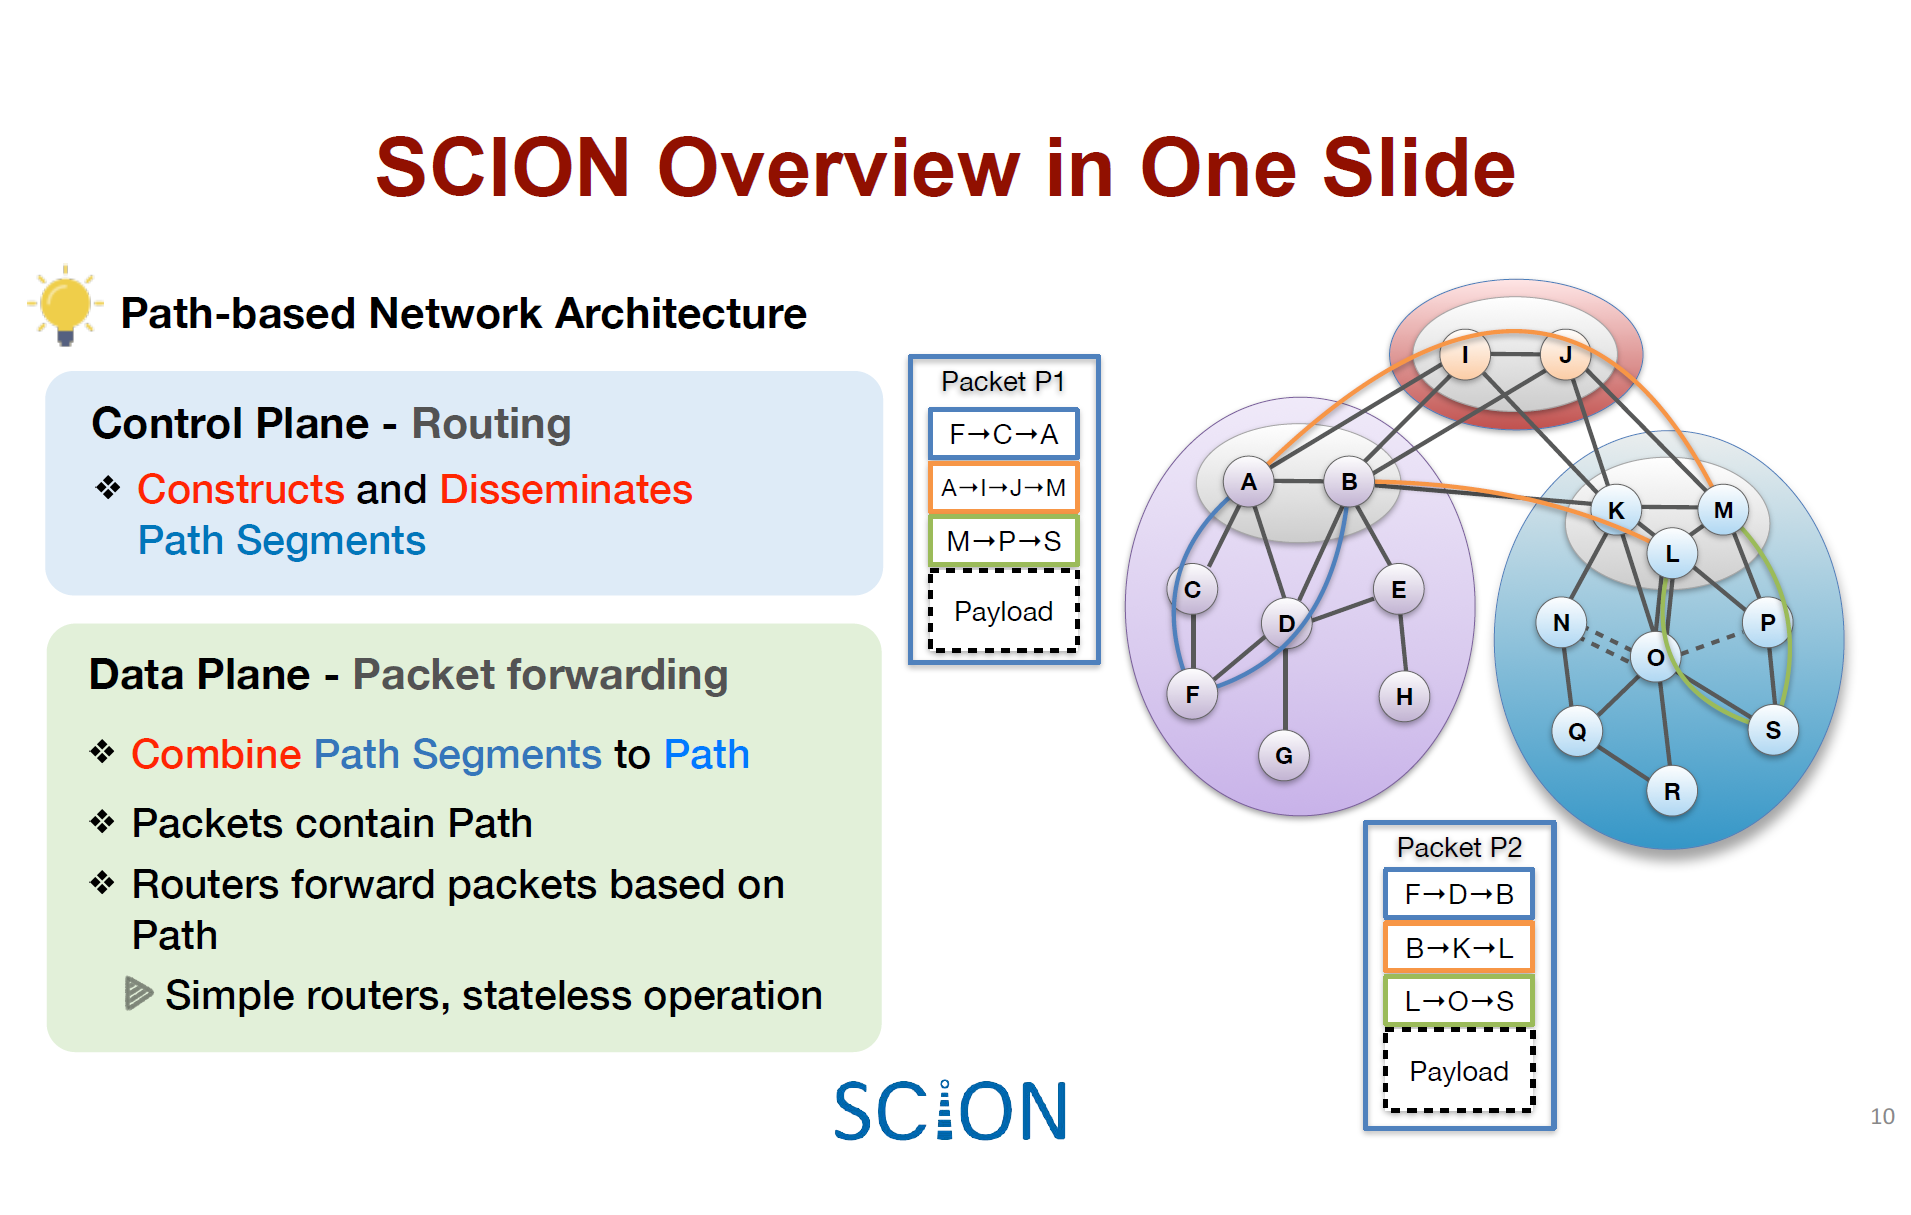
\includegraphics[width=\linewidth]{Figures/SCION_overview.PNG} 
\end{minipage}


\subsubsection{Intra-ISD Path Exploration: Beaconing}
Beaconing is am asynchronous process through which paths are found in SCION. The Core ASes in an ISD (Isolation Domain) periodically flood the ISD with PCBs, by sending them in an anycast fashion (dubbed service anycast in SCION). Any AS receiving this packet will send it to its beacon server, which will add the current AS info and send the PCB to the ASes downstream. When beacons reach leaf nodes in the AS graph, the process is completed. Each AS receives multiple PCBs representing path segments to a core AS.\\

Each AS deploys one or multiple beacon servers. SCION border routers receive PCB
and select one beacon server to forward it to. Beacon servers coordinate to resend PCBs periodically to downstream ASes (currently every 5 seconds). ASes can choose to which customers and peers to forward which beacons, but in the end it is the sources that determine the final path.\\

\textbf{PCB contents:} PCB contains an info field with: PCB creation time. Each AS on path adds: AS name, Hop field for data-plane forwarding (Link identifiers, Expiration time, Message Authentication Code (MAC)), AS signature.\\
\textit{Link identifier}: ASes have multiple interface numbers. The hop field has an \texttt{IN} and \texttt{OUT} link identifier, they say where traffic enters/ leaves the AS.\\
\textit{MAC}: highly efficient (verified in a few ns) but needs symmetric keys (only known inside the AS). This allows the AS to verify its own forwarding information.

\textbf{Up-Path and Down-Path Segments:} PCBs contain path segments that
can be used as communication paths. A path segment is any contiguous subsequence of ASes contained in a PCB, provided that at least one of the extremes is a core AS. They owe their name to the fact that they represent different segments of a whole path. Each path is comprised of an \textbf{up-path segment} (from source AS to a core AS) plus a \textbf{core-path segment} (from core AS to core AS, possibly on a different ISD), plus a \textbf{down-path segment} (from core to destination AS).\\

\subsubsection{Core Beaconing for Inter-ISD Path Exploration}
Beaconing that happens inside ISDs also happens across ISDs $\rightarrow$ core ASes beacon among each other. Beacon info looks similar as for intra ISD beaconing. With Core Beaconing for Inter-ISD Path Exploration, there is \textit{no} convergence process! Connecting the whole internet would only take a few seconds. However, finding the best and multiple paths takes longer.\\
\textit{But:} scalability of inter-ISD beaconing is actually \textbf{worse} than in BGP because we send lots of inter-ISD beacons and we also want to discover multiple paths. However, it still scales since the number of core ASes is highly limited (few tier 1 Ases).

\subsubsection{Path server infrastructure}
Every AS has its own path server. Non-core AS's path server contains up-path segments to reach the core ASes. Core AS's path server contains down-path segments and core-path segments. Caches along the way cache paths at various levels.\\
\textbf{Up-Path Segment Registration:} AS selects path segments to announce
as up-path segments for local hosts. Up-path segments are registered at local path servers.\\
\textbf{Down-Path Segment Registration:} AS selects path segments to announce as down-path segments for others to use to communicate with AS. Down-path segments are uploaded to core path server in core AS.

\subsection{Data plane: How to send packets}
In IP, the router looks up a routing table and (usually based on the destination of the packet) makes a routing decision, forwarding the packet to the appropriate interface. In SCION none of that happens: the packet already contains the forwarding information (full AS path), so a router only needs to check the next hop information in the SCION header. As a consequence, SCION packets need larger headers compared to IP.

\subsubsection{Path lookup}
Disadvantage of SCION over today's internet: we need to look up paths. In today's internet, we just lookup an IP, send a packet and pray.\\

\paragraph{Steps of a host to obtain path segments:}
\begin{enumerate}
	\item Host contacts RAINS server with a name: H $\rightarrow$ RAINS\\
	RAINS $\rightarrow$ H: ISD X, AS Y, local address Z
	\item Host contacts local path server to query path segments H $\rightarrow$→ PS: ISD X, AS Y\\
	PS $\rightarrow$ H: up-path (to local ISD core ASes), core-path (connect up-path and down-path
	segments), down-path segments (from core AS to ISD X)
	\item Host combines path segments to obtain end-to-end 	paths, which are added to packets\\
\end{enumerate}

\textbf{Path lookup: local ISD}\\
In step 2, client requests path segments from local path server. If down-path segments are not cached, local path server sends request to core path server.\\

\textbf{Path Lookup: remote ISD}\\
In step 2, client requests path segments from local path server. If down-path segments are not cached, local path server send request to core path server. If core path server does not have path segments cached, it will contact remote core path server.

Path segments are valid for several hours and cached locally. Otherwise the whole process would take too much time for each time we want to send. SCION’s path combination of up-path, core-path, and down-path segments reflect current Internet routing.\\

Problem: Economic incentives are not all prevailed in SCION: customer could choose to use a very costly link (path) since we have multiple paths available. This would be bad for the provider. \textit{But:} this could be solved by the provider by setting BW limits or just making customers pay more if they use more expensive links.

\begin{minipage}{\linewidth}
    \centering      
    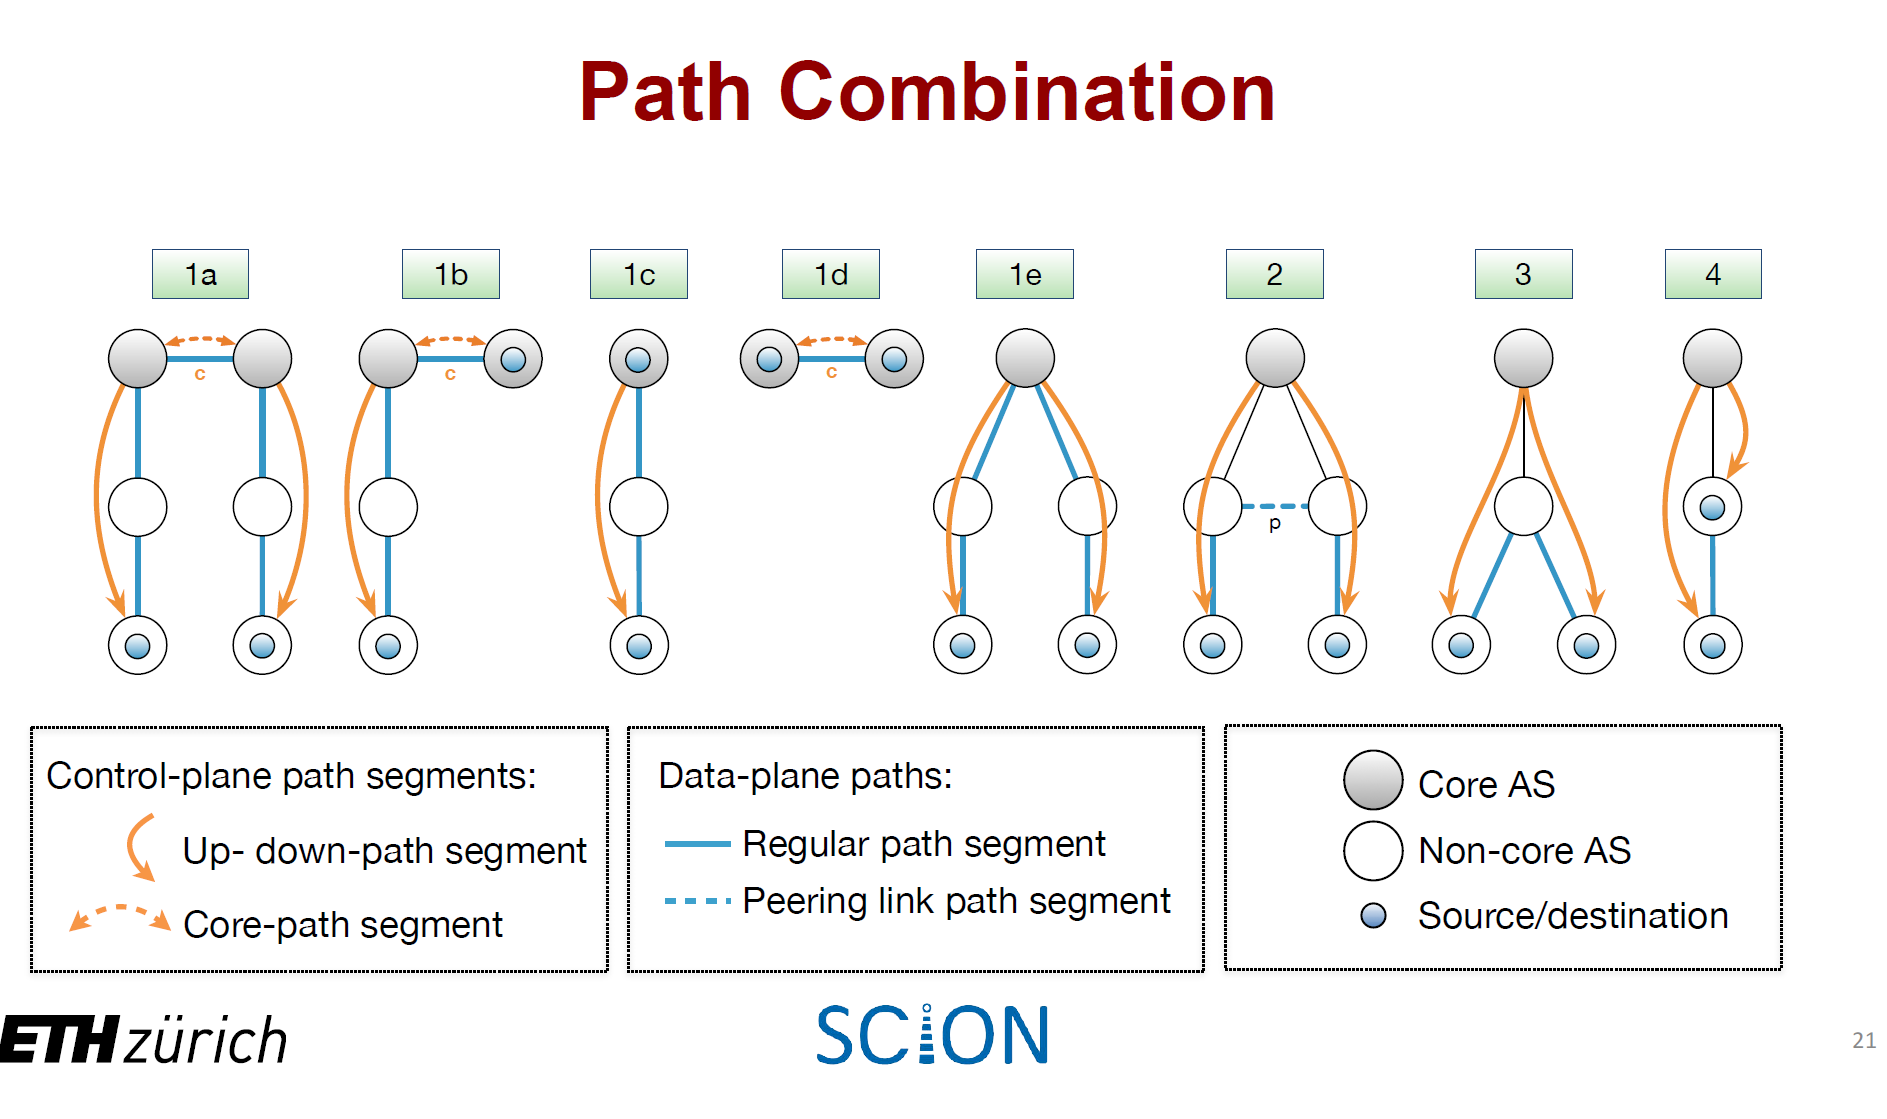
\includegraphics[width=\linewidth]{Figures/SCION_pathcombination.PNG} 
\end{minipage}

\subsubsection{SCION Packet Header}
A SCION packet has multiple headers:

\begin{itemize}
	\item SCION common header
	\item SCION source and destination address
	\item Info field provides information about a path segment
	\item Path segment consists of one or multiple hop fields
\end{itemize}

SCION does not look at srcIP \& dstIP in the network! Only when the packet gets to the destination AS will IPs be considered. \textbf{This allows for communication between private address spaces!} E.g. 192.168.0.1 in AS X could communicate with 192.168.0.1 in AS Y. Also, this would solve IPv4 address exhaustion (although IPv6 already solved it).

\begin{minipage}{\linewidth}
    \centering      
    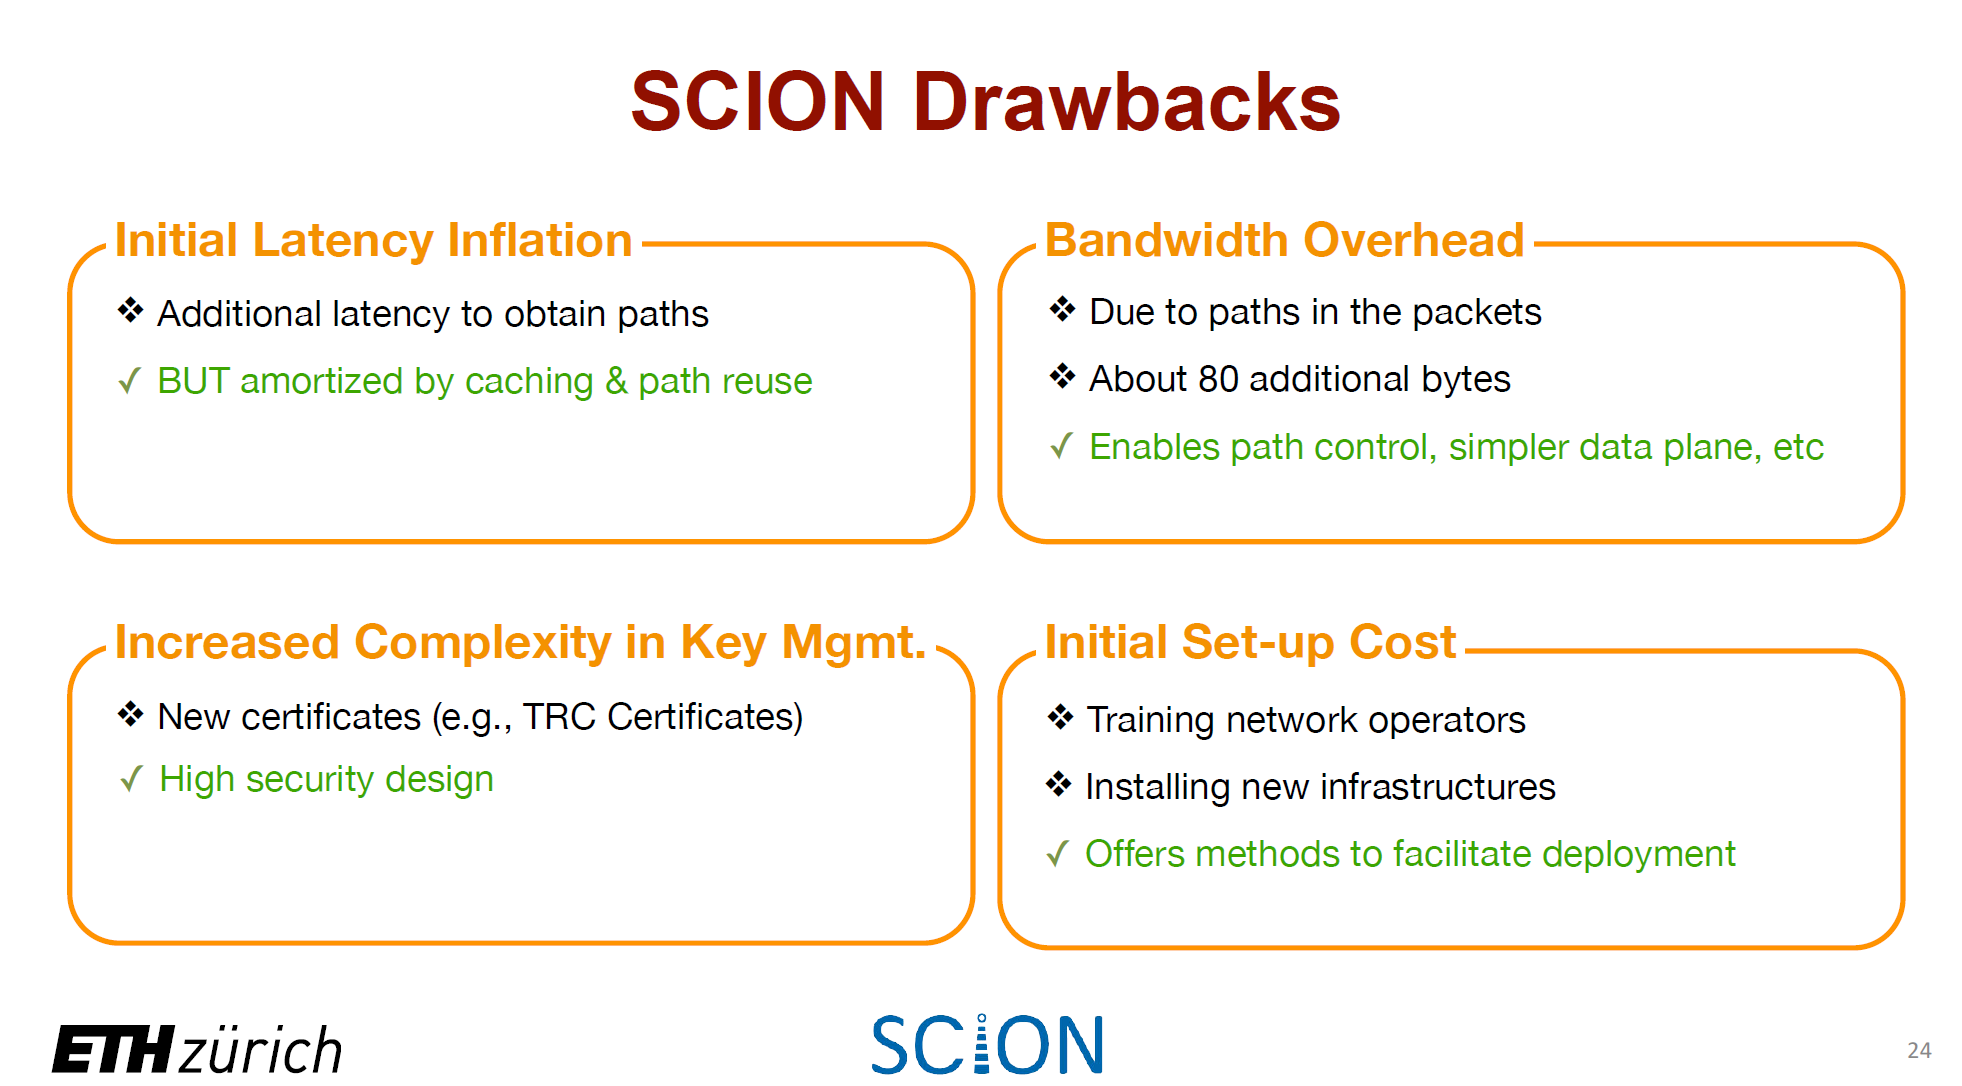
\includegraphics[width=\linewidth]{Figures/SCION_drawbacks.PNG} 
\end{minipage}

\subsubsection{Ingress and Egress Interface Identifiers}

Each AS assigns a unique integer identifier to each interface that connects to a neighboring A. The interface identifiers identify ingress/egress links for traversing AS. ASes use internal routing protocol to find route from ingress SCION border router to egress SCION border router

\subsubsection{Path Encoding in Packet}

In order to send a packet back (destination to source), we don't need to do another path lookup! The dst just needs to do some parsing to reverse the path. Forward and return paths are the same (one could also lookup a new path).

\subsubsection{Hop Field MAC Verification}

Message Authentication Code (MAC) computation and verification of Hop Field MAC value based on local AS secret key (not shared with any external entity).\\
Computation: $MAC_K(Timestamp,Flags’_{HF},ExpTime,Ingress,Egress, HF’)$, with HF the hop field of the previous AS.\\
With AESni HW crypto, only ~30 cycles are needed to compute MAC!

\subsection{Deployment and use cases}

\paragraph{ISP deployment:} Core ASes have to adapt quite a lot and need to do quite a bit of work for SCION. For regular ASes, most of this work is not needed. Integration of SCION limits to additional infrastructure such as beacon server, path server, RAINS, certificate, SIBRA and time servers.

\subsubsection{Use Case: Low-Latency Connectivity}

Generally, two paths exist between Europe and Southeast Asia: 

\begin{itemize}
	\item western route (Europe-US-SEA): High latency, high bandwidth
	\item eastern route (Europe, Suez canal, SEA): Low latency, low bandwidth
\end{itemize}

BGP is a “money routing protocol”, traffic follows cheapest path, typically highest bandwidth path. Thus, Europe-SEA traffic generally takes the western route. There is no wrong path (both have advantages and disadvantages) but the wrong thing to do is to only advertise one single path (as BGP does).

\subsubsection{Use Case: Low Earth Orbit Satellite Networks}

Speed of light in fibres is a lot slower than speed of light in free space. New Low Earth Orbit (LEO) satellite networks only require around 5ms propagation latency between earth and satellite. Inter-Satellite Laser (ISL) links enable global communication. However, LEO has frequent outages/ short time windows of availability due to changing weather conditions - BGP convergence is too slow to support. SCION however can optimally integrate LEO network into Internet fabric.
